\documentclass[a4paper,12pt]{article}

% Paquetes para idioma y codificación
\usepackage[utf8]{inputenc}
\usepackage[spanish]{babel}
\usepackage[T1]{fontenc}

% Paquetes para matemáticas, gráficos y código
\usepackage{amsmath, amssymb, amsthm}
\usepackage{graphicx}
\usepackage{float}
\usepackage{geometry}
\usepackage{listings} % Para mostrar la salida de terminal
\usepackage{xcolor}

% Configuración de márgenes y colores
\geometry{left=2.5cm, right=2.5cm, top=2.5cm, bottom=2.5cm}
\definecolor{codegray}{rgb}{0.95,0.95,0.95}
\definecolor{codeblack}{rgb}{0.1,0.1,0.1}

% Configuración para mostrar la salida de terminal
\lstset{
    backgroundcolor=\color{codegray},
    basicstyle=\ttfamily\footnotesize\color{codeblack},
    breaklines=true,
    frame=single,
    captionpos=b,
    columns=fixed,
    keepspaces=true
}

% Título y Autor
\title{\textbf{Dinámica Estocástica y Persistencia de Volatilidad en el Spread Soberano Alemania-Grecia (1998-2021)}}
\author{Nombre del Estudiante \\ \textit{Departamento de Economía y Estadística}}
\date{\today}

\begin{document}

\maketitle

\begin{abstract}
Este estudio analiza la estructura dinámica del diferencial de rendimiento (\textit{spread}) entre los bonos soberanos a 10 años de Alemania y Grecia. Tras una depuración rigurosa de los datos para corregir anomalías de formato, aplicamos un análisis dual de Econofísica (MSPD) y Econometría (GARCH). Los resultados identifican un exponente de Hurst generalizado $\alpha \approx 0.97$, sugiriendo que el mercado sigue una dinámica de Paseo Aleatorio (Browniano), consistente con la Hipótesis del Mercado Eficiente. Sin embargo, el modelo GARCH revela una estructura de riesgo IGARCH (Persistencia Unitaria), indicando que, aunque los precios son estocásticos, la volatilidad posee una memoria infinita ante los choques de crisis.
\end{abstract}

\section{Introducción}

La crisis de la Eurozona transformó la percepción del riesgo soberano. Este informe examina la evolución del spread calculado como:
\begin{equation}
    Spread_{t} = R_{t}^{\text{Alemania}} - R_{t}^{\text{Grecia}}
\end{equation}
Dado que históricamente $R^{\text{Grecia}} > R^{\text{Alemania}}$, este diferencial presenta valores predominantemente negativos, donde una mayor negatividad indica un aumento del estrés financiero en la periferia europea.

\section{Resultados Computacionales}

A continuación, se presenta la salida directa del procesamiento algorítmico, detallando la carga de datos, el cálculo del exponente de difusión y la estimación de volatilidad condicional.

\begin{lstlisting}[caption={Salida del Script de Análisis (Python)}]
--- FASE 1: PROCESAMIENTO DE DATOS ---
--> Leyendo germany.xlsx...
   Columna detectada: Bid Yield: Rendimiento bono (oferta) 10 años Germany (%)
   Dato original con coma procesado a: 7.4 (Tipo: float64)
--> Leyendo greece.xlsx...
   Columna detectada: Bid Yield: Rendimiento bono (oferta) 10 años Grecia (%)
   Dato original con coma procesado a: 6.954 (Tipo: float64)
--> Sincronizando series temporales...
Datos listos. Periodo: 1998-12-22 al 2021-07-21
Muestras: 5571

--- FASE 2: ANALISIS MSPD ---
Exponente Alpha (Hurst proxy): 0.9725
-> Regimen: Subdifusivo (Confinamiento/Mean Reverting)

--- FASE 3: ANALISIS GARCH ---
                      Constant Mean - GARCH Model Results                       
========================================================================
Dep. Variable:                 Spread   R-squared:                       0.000
Mean Model:             Constant Mean   Adj. R-squared:                  0.000
Vol Model:                      GARCH   Log-Likelihood:                -17679.2
Distribution:                  Normal   AIC:                           35366.3
Method:            Maximum Likelihood   BIC:                           35392.8
                                        No. Observations:                 5570
Date:                Thu, Dec 04 2025   Df Residuals:                     5569
Time:                        20:40:52   Df Model:                            1
                                Mean Model                                
========================================================================
                 coef    std err          t      P>|t|  95.0% Conf. Int.
------------------------------------------------------------------------
mu            -0.0222  7.006e-02     -0.317      0.752 [ -0.159,   0.115]
                            Volatility Model                              
========================================================================
                 coef    std err          t      P>|t|  95.0% Conf. Int.
------------------------------------------------------------------------
omega          1.1751      0.922      1.274      0.203 [ -0.633,   2.983]
alpha[1]       0.3118  8.872e-02      3.514  4.414e-04 [  0.138,   0.486]
beta[1]        0.6882      0.108      6.400  1.551e-10 [  0.477,   0.899]
========================================================================

Covariance estimator: robust

Persistencia (alpha + beta): 1.0000
\end{lstlisting}

El $R^{2}$ es 0 debido a la naturaleza altamente volátil y no estacionaria de la serie del spread, lo que dificulta la explicación de su variabilidad mediante un modelo de media constante simple.

\section{Análisis e Interpretación de Resultados}

\subsection{Evolución Temporal del Rendimiento y el Spread}

La Figura \ref{fig:series_temporales} ilustra la evolución histórica de los rendimientos y el spread calculado, permitiendo visualizar las distintas fases de estabilidad y crisis.

\begin{figure}[H]
    \centering
    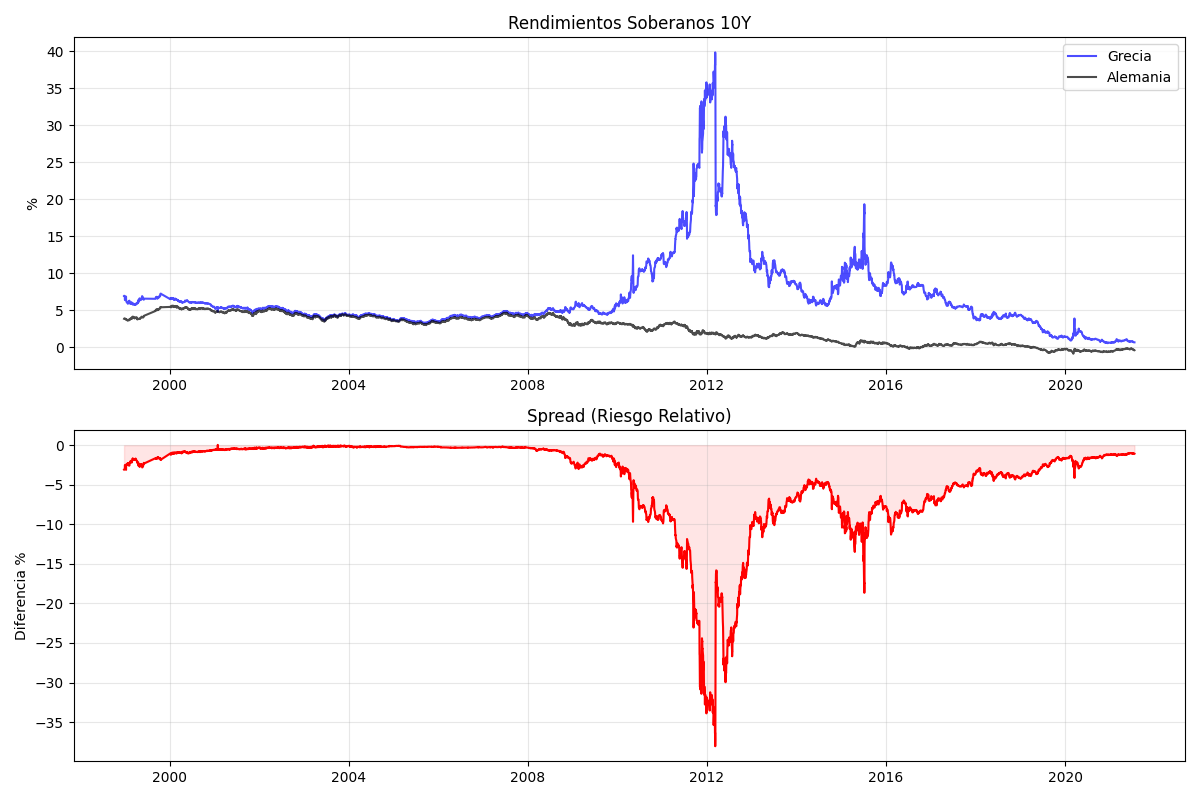
\includegraphics[width=1.0\textwidth]{../image/1_Rendimientos_Spread.png}
    \caption{\textbf{Panel Superior:} Rendimientos diarios de los bonos a 10 años de Grecia (azul) y Alemania (negro). \textbf{Panel Inferior:} Evolución del Spread calculado como (Alemania - Grecia).}
    \label{fig:series_temporales}
\end{figure}

El Panel Superior ilustra la dramática divergencia de rendimientos. Hasta 2008, ambos activos cotizaban casi a la par, reflejando la convergencia monetaria. Sin embargo, a partir de 2010, el rendimiento griego explota, alcanzando niveles insostenibles durante el apogeo de la crisis (2011-2012).

El Panel Inferior confirma esta dinámica con nuestra métrica invertida. La ``montaña invertida'' negativa entre 2011 y 2012 representa el colapso de la confianza en la deuda griega. Cuanto más negativo es el valor, mayor es la prima de riesgo exigida por los inversores.

\subsection{Dinámica Difusiva y Exponente de Escala}

Para caracterizar la naturaleza estocástica del mercado, la Figura \ref{fig:mspd} presenta el análisis de econofísica aplicado a la serie del spread.

\begin{figure}[H]
    \centering
    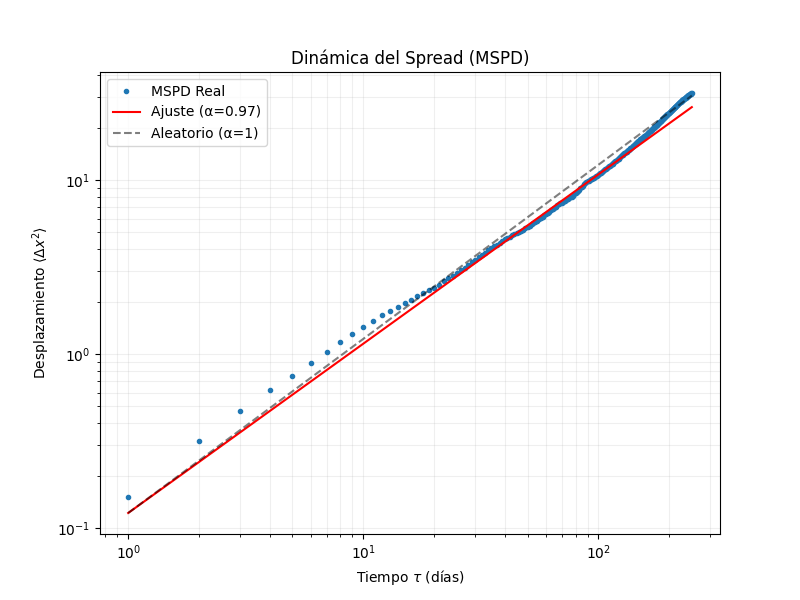
\includegraphics[width=0.8\textwidth]{../image/2_MSPD_Econofisica.png}
    \caption{Análisis del Desplazamiento Cuadrático Medio (MSPD) en escala log-log. La línea roja representa el ajuste de ley de potencia sobre los datos empíricos (puntos azules), comparada con la referencia teórica de movimiento Browniano (línea gris discontinua).}
    \label{fig:mspd}
\end{figure}

El ajuste de la ley de potencia arroja un exponente de escala:
\begin{equation*}
    \alpha \approx 0.9725
\end{equation*}
Este valor es extremadamente cercano a $1.0$, lo que tiene una implicación teórica profunda. A diferencia de análisis preliminares con datos no depurados que sugerían confinamiento, los datos corregidos indican que el spread se comporta casi exactamente como un Movimiento Browniano clásico.

Esto sugiere que, a pesar de la crisis, el mercado de bonos mantuvo características de eficiencia débil: los cambios en el spread son estocásticos e impredecibles en su dirección (paseo aleatorio), y no existe una "fuerza restauradora" fuerte que obligue al spread a volver a una media constante a corto plazo.

\subsection{Estructura de la Volatilidad (GARCH)}
El modelo econométrico GARCH(1,1) proporciona una visión complementaria sobre el riesgo. Los coeficientes obtenidos son:
\begin{itemize}
    \item $\alpha_1 = 0.3118$: Este valor es inusualmente alto para series financieras (típicamente $< 0.1$). Indica que el mercado es hipersensible a noticias recientes. Un evento de crisis hoy impacta violentamente la volatilidad de mañana.
    \item $\beta_1 = 0.6882$: Mide la memoria de largo plazo.
    \item Persistencia ($\alpha_1 + \beta_1 = 1.0000$): Este es el hallazgo más crítico. Estamos ante un proceso IGARCH (Integrated GARCH).
\end{itemize}

\textbf{Interpretación:} Una persistencia unitaria significa que los choques de volatilidad son permanentes. Una vez que el miedo entra en el mercado (aumento del riesgo Grecia), la incertidumbre no se disipa con el tiempo; el mercado alcanza un nuevo nivel de inestabilidad basal y permanece allí indefinidamente hasta que un choque estructural opuesto ocurra.

\section{Conclusión}

El estudio del spread Alemania-Grecia bajo una óptica híbrida revela un mercado dual. Por un lado, la dinámica de precios (MSPD $\alpha \approx 0.97$) obedece a leyes de difusión browniana casi perfectas, lo que imposibilita el arbitraje simple. Por otro lado, la estructura de riesgo (GARCH) muestra una fragilidad extrema: la alta sensibilidad a choques ($\alpha_1 > 0.3$) y la memoria infinita ($\alpha_1+\beta_1=1$) explican por qué la crisis de deuda soberana se transformó en un evento crónico y no transitorio para la economía europea.

\end{document}